\documentclass[a0paper,portrait]{baposter}
\usepackage[french]{babel}


\usepackage{wrapfig}
\usepackage{lmodern}
\usepackage{lipsum,graphicx}
\usepackage{fontspec}
\usepackage{advdate}
\usepackage{svg}
\usepackage{xcolor}
\usepackage{tabularx}
\usepackage{enumitem}


% Set main font (Abraham)
% \setmainfont[
%     Path = font/Abraham/,
%     Extension = .otf,
%     % SmallCapsFont = *-smallcaps,
%     BoldFont = *-bold, % Outline
%     ItalicFont = *-italic, % Italic
%     BoldItalicFont = *-bolditalic % Outline Italic
% ]{abraham}
% \setmainfont{TeX Gyre Termes}

%

\graphicspath{{figures/}} % Directory in which figures are stored

\newcommand{\compresslist}{%
\setlength{\itemsep}{0pt}%
\setlength{\parskip}{1pt}%
\setlength{\parsep}{0pt}%
}

\newenvironment{boenumerate}
  {\begin{enumerate}\renewcommand\labelenumi{\textbf\theenumi.}}
  {\end{enumerate}}


\begin{document}

\definecolor{Mycolor1}{HTML}{3FFF00}
\definecolor{Mycolor2}{HTML}{0FF000} %0FF000

\begin{poster}
{
grid=false,
headerborder=open, % Adds a border around the header of content boxes
colspacing=1em, % Column spacing
bgColorOne=white, % Background color for the gradient on the left side of the poster
bgColorTwo=white, % Background color for the gradient on the right side of the poster
borderColor=Mycolor1, % Border color
headerColorOne=Mycolor2, % Background color for the header in the content boxes (left side)
headerColorTwo=Mycolor2, % Background color for the header in the content boxes (right side)
headerFontColor=white, % Text color for the header text in the content boxes
boxColorOne=white, % Background color of the content boxes
textborder=rounded, %rectangle, % Format of the border around content boxes, can be: none, bars, coils, triangles, rectangle, rounded, roundedsmall, roundedright or faded
eyecatcher=false, % Set to false for ignoring the left logo in the title and move the title left
headerheight=0.08\textheight, % Height of the header
headershape=rounded, % Specify the rounded corner in the content box headers, can be: rectangle, small-rounded, roundedright, roundedleft or rounded
headershade=plain,
headerfont=\Large\textsf, % Large, bold and sans serif font in the headers of content boxes
%textfont={\setlength{\parindent}{1.5em}}, % Uncomment for paragraph indentation
linewidth=1pt % Width of the border lines around content boxes
}
{}
%
%----------------------------------------------------------------------------------------
%	TITLE AND AUTHOR NAME
%----------------------------------------------------------------------------------------
%
{\textsf{{Tableau de bord - Éco-marathon Shell 2023}}} % Titre en Sans Serif
{\sf\vspace{0.1em}\\
Électrique  -  {\AdvanceDate[0]\today} 
\vspace{0.1em}\\
\small{ Période couverte du {\AdvanceDate[-7]\today} au {\AdvanceDate[0]\today}
}
}
{
\includegraphics[width=.1\linewidth]{img/udes.pdf}} % TU Dublin logo

\headerbox{Objectif de projet}{name=objectif,column=0,row=0, span=3}{
Créer un véhicule efficace à propulsion électrique pour gagner la compétition de l'Éco-marathon Shell dans la division ``véhicule urbain'' en 2023.

\vspace{0.2cm} %vertical spacing
}


% \headerbox{Objectifs de session}{name=objectif_session,column=1,below=objectif,span=2}{

% %\vspace{0.15cm}
% \centering
% {    \begin{tabularx}{\linewidth}{
        >{\hsize=1.5\hsize}X
        >{\hsize=1.0\hsize}X
        >{\centering\arraybackslash\hsize=0.5\hsize}X
      }
        
        \textbf{Objectif} & \textbf{Système} & \textbf{Avancement} \\
         Modélisation numérique & Moteur/Transmission & 100\% \\
         CAD détaillé & Moteur/Transmission & 90\% \\
         Assemblage V0 & Moteur/Transmission & 15\% \\
         PCB V2 onduleur fonctionnel & Onduleur & 60\% \\
         Arbre alimentation fonctionnel & Onduleur & 60\% \\
         BMS V2 testé & Bloc batterie & 30\% \\
         Bloc batterie V0 assemblé et testé & Bloc batterie & 85\% \\
         Instrumentation testée & Instrumentation & 25\% \\
      \end{tabularx}
    
        
     % Template des Objectifs rencontés:
     %
     % Objectif : l'objectif de la session
     % Système  : le nom ou numéro système que l'objectif touche ex: Simulateur ou SIM1
     % &  & = ESPACE POUR LE FORMATAGE NE PAS ENLEVER
     % Avancement : Pourcentage estimé d'avancement de l'objectif.
     %
     %  
     %  \textbf{Objectif} & \textbf{Système} &  & \textbf{Avancement}\\
     %   Objectif & Système &  & Avancement \\
     %   Objectif & Système &  & Avancement \\
     %   Objectif & Système &  & Avancement \\
     %   Objectif & Système &  & Avancement \\
     %   Objectif & Système &  & Avancement \\
    
    
    
    
    
}

% % \vspace{0.4cm} % spacing vertical

% }

\headerbox{Ordre du jour}{name=ordre_jour,column=0,below=objectif,span=2}{
\vspace{0.1cm}
\begin{itemize}
    \item \textbf{Rencontre gestion:}
    \begin{enumerate}
        \item Présentation du tableau de bord
        \item Planification détaillée S8
        \item Analyse de risque
    \end{enumerate}
\end{itemize}
\vspace{0.20cm} % spacing vertical
}

\headerbox{Membres}{name=membres,column=2,below=objectif,span=1}{
\vspace{0.3cm}


% inserts an image inside the box, 5 rows high | r = on the right along side text 
\begin{wrapfigure}[5]{r}{0.25\textwidth}
\includegraphics[width=0.9\linewidth]{img/membres/François-Paquette-3.jpg} 
\end{wrapfigure}
\subsubsection*{}
\vspace{-2mm}
\textbf{François Paquette}

Bloc batterie

Moteur / Transmission

\begin{wrapfigure}[5]{r}{0.25\textwidth}
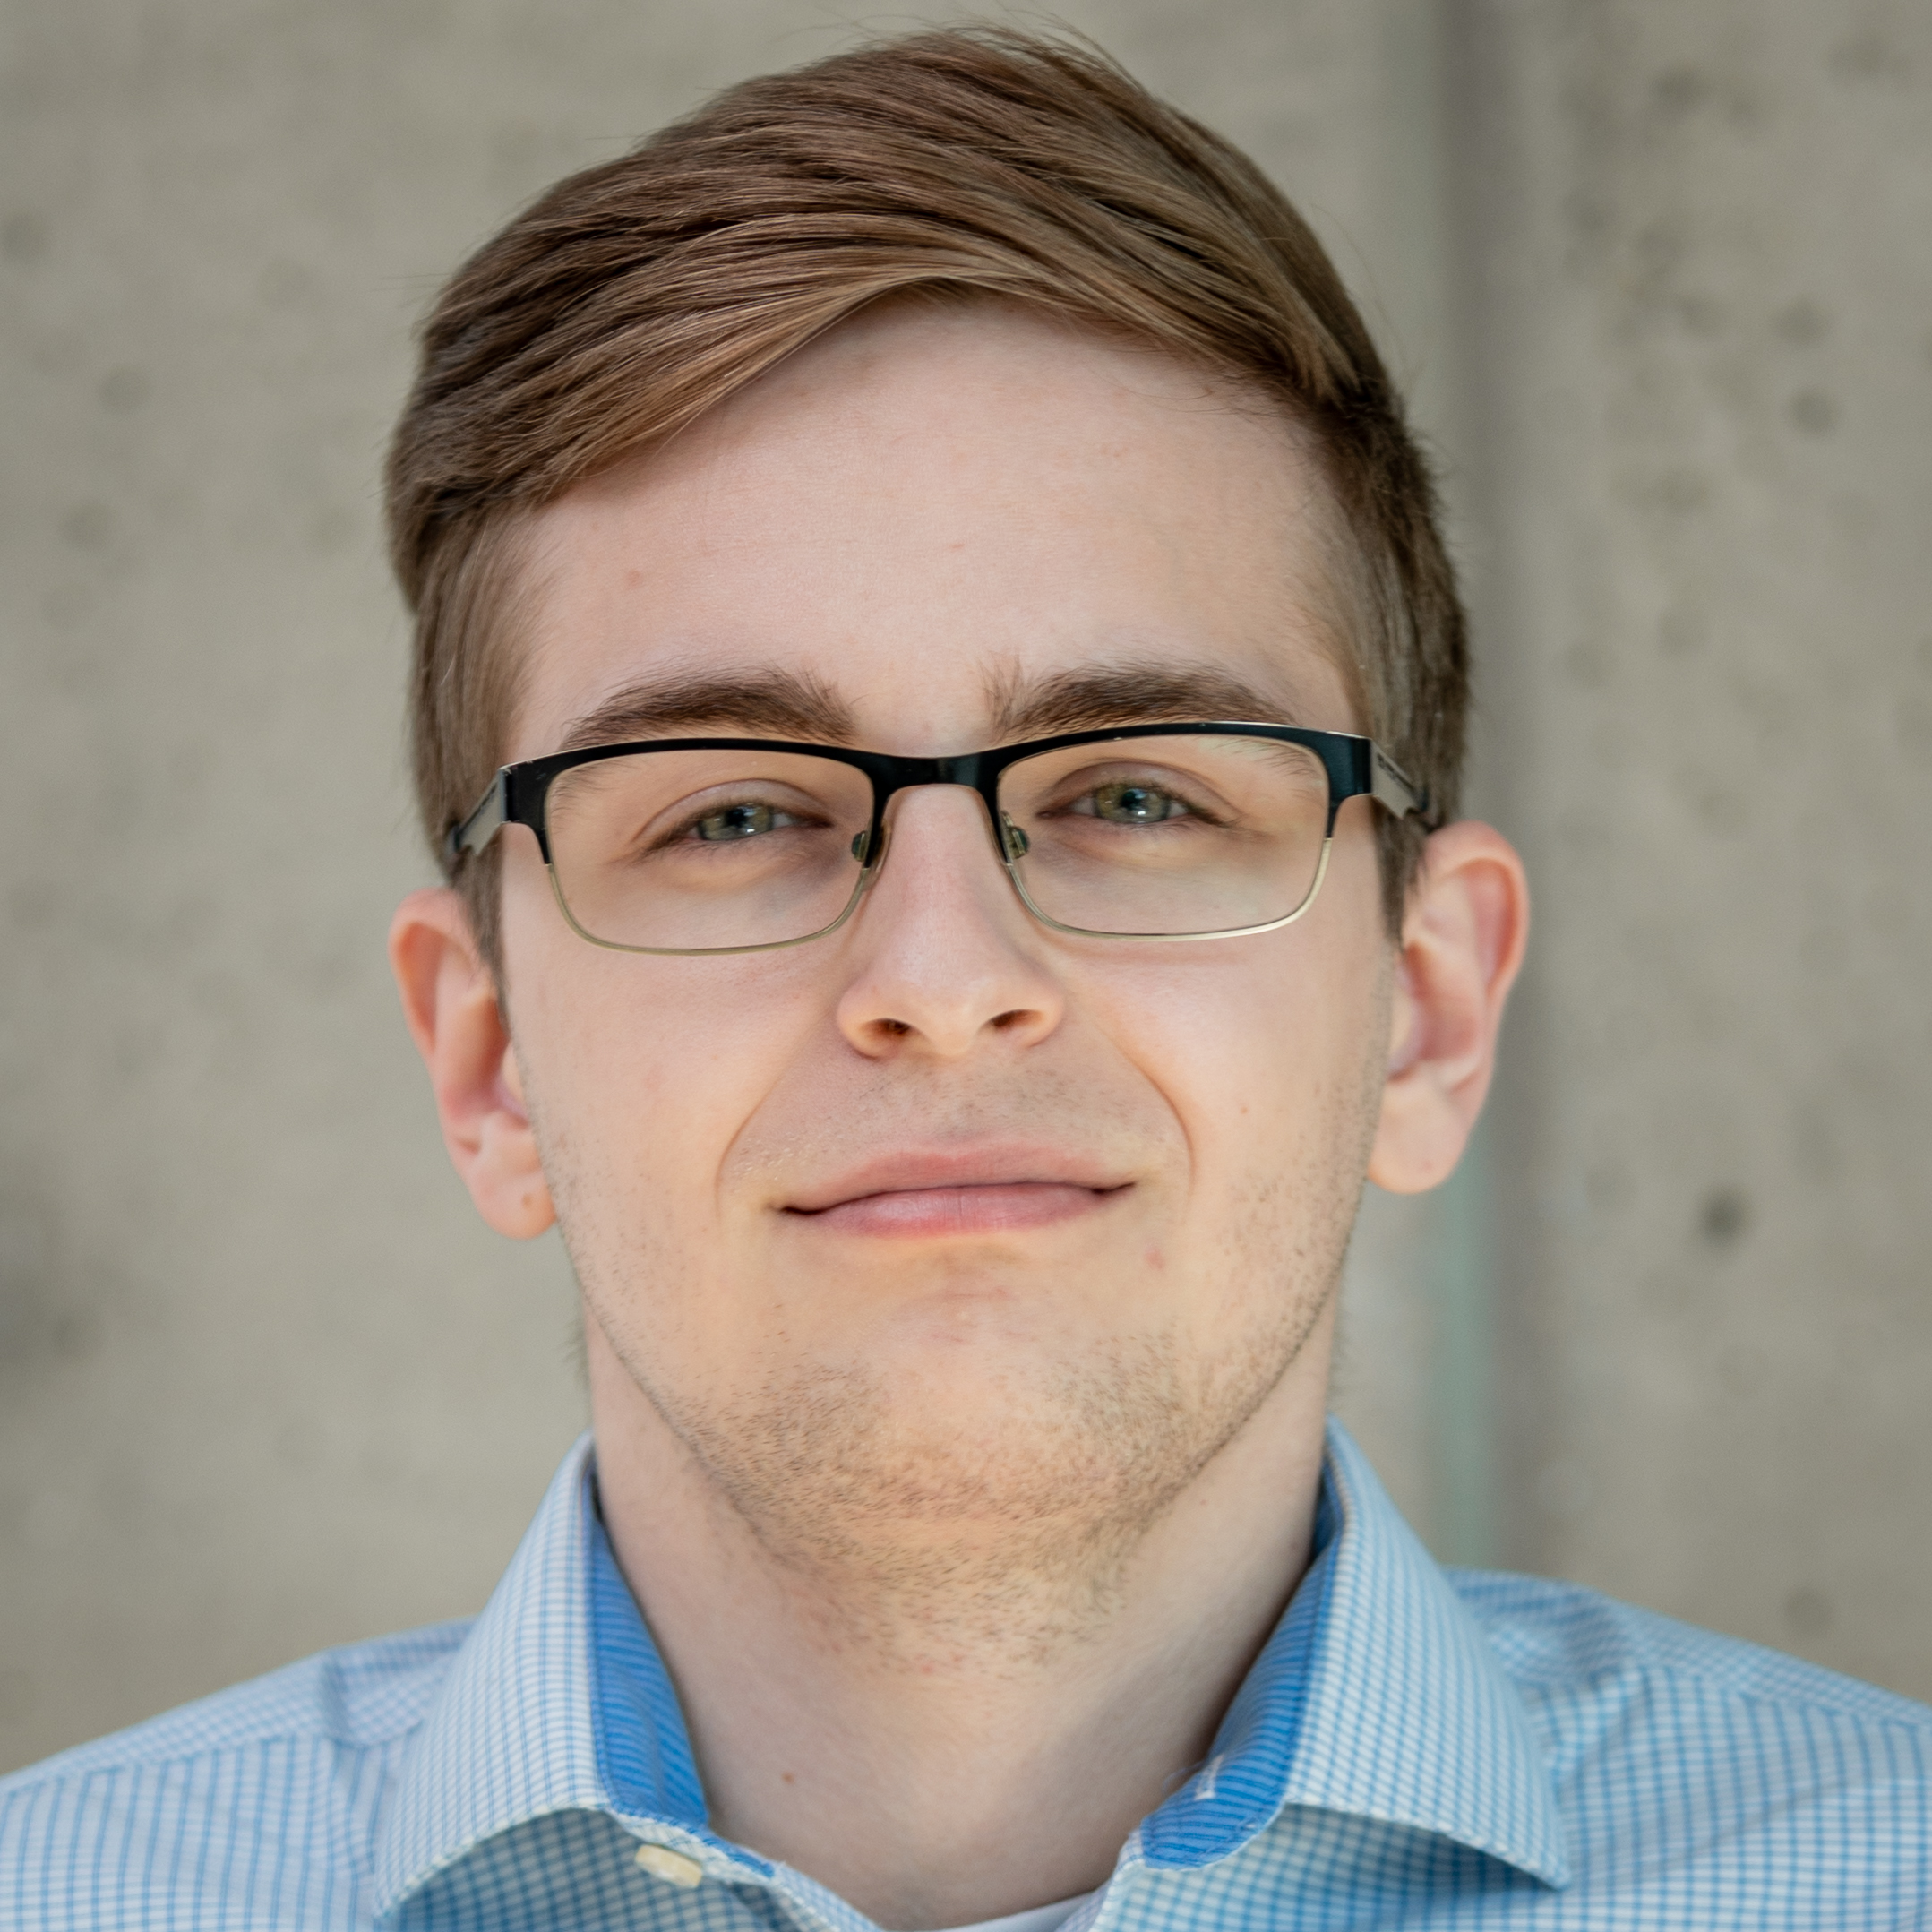
\includegraphics[width=.9\linewidth]{img/membres/Gabriel-Cabana-2.jpg} 
\end{wrapfigure}
\subsubsection*{}
\vspace{2mm}
\textbf{Gabriel Cabana}

Moteur

\begin{wrapfigure}[5]{r}{0.25\textwidth}
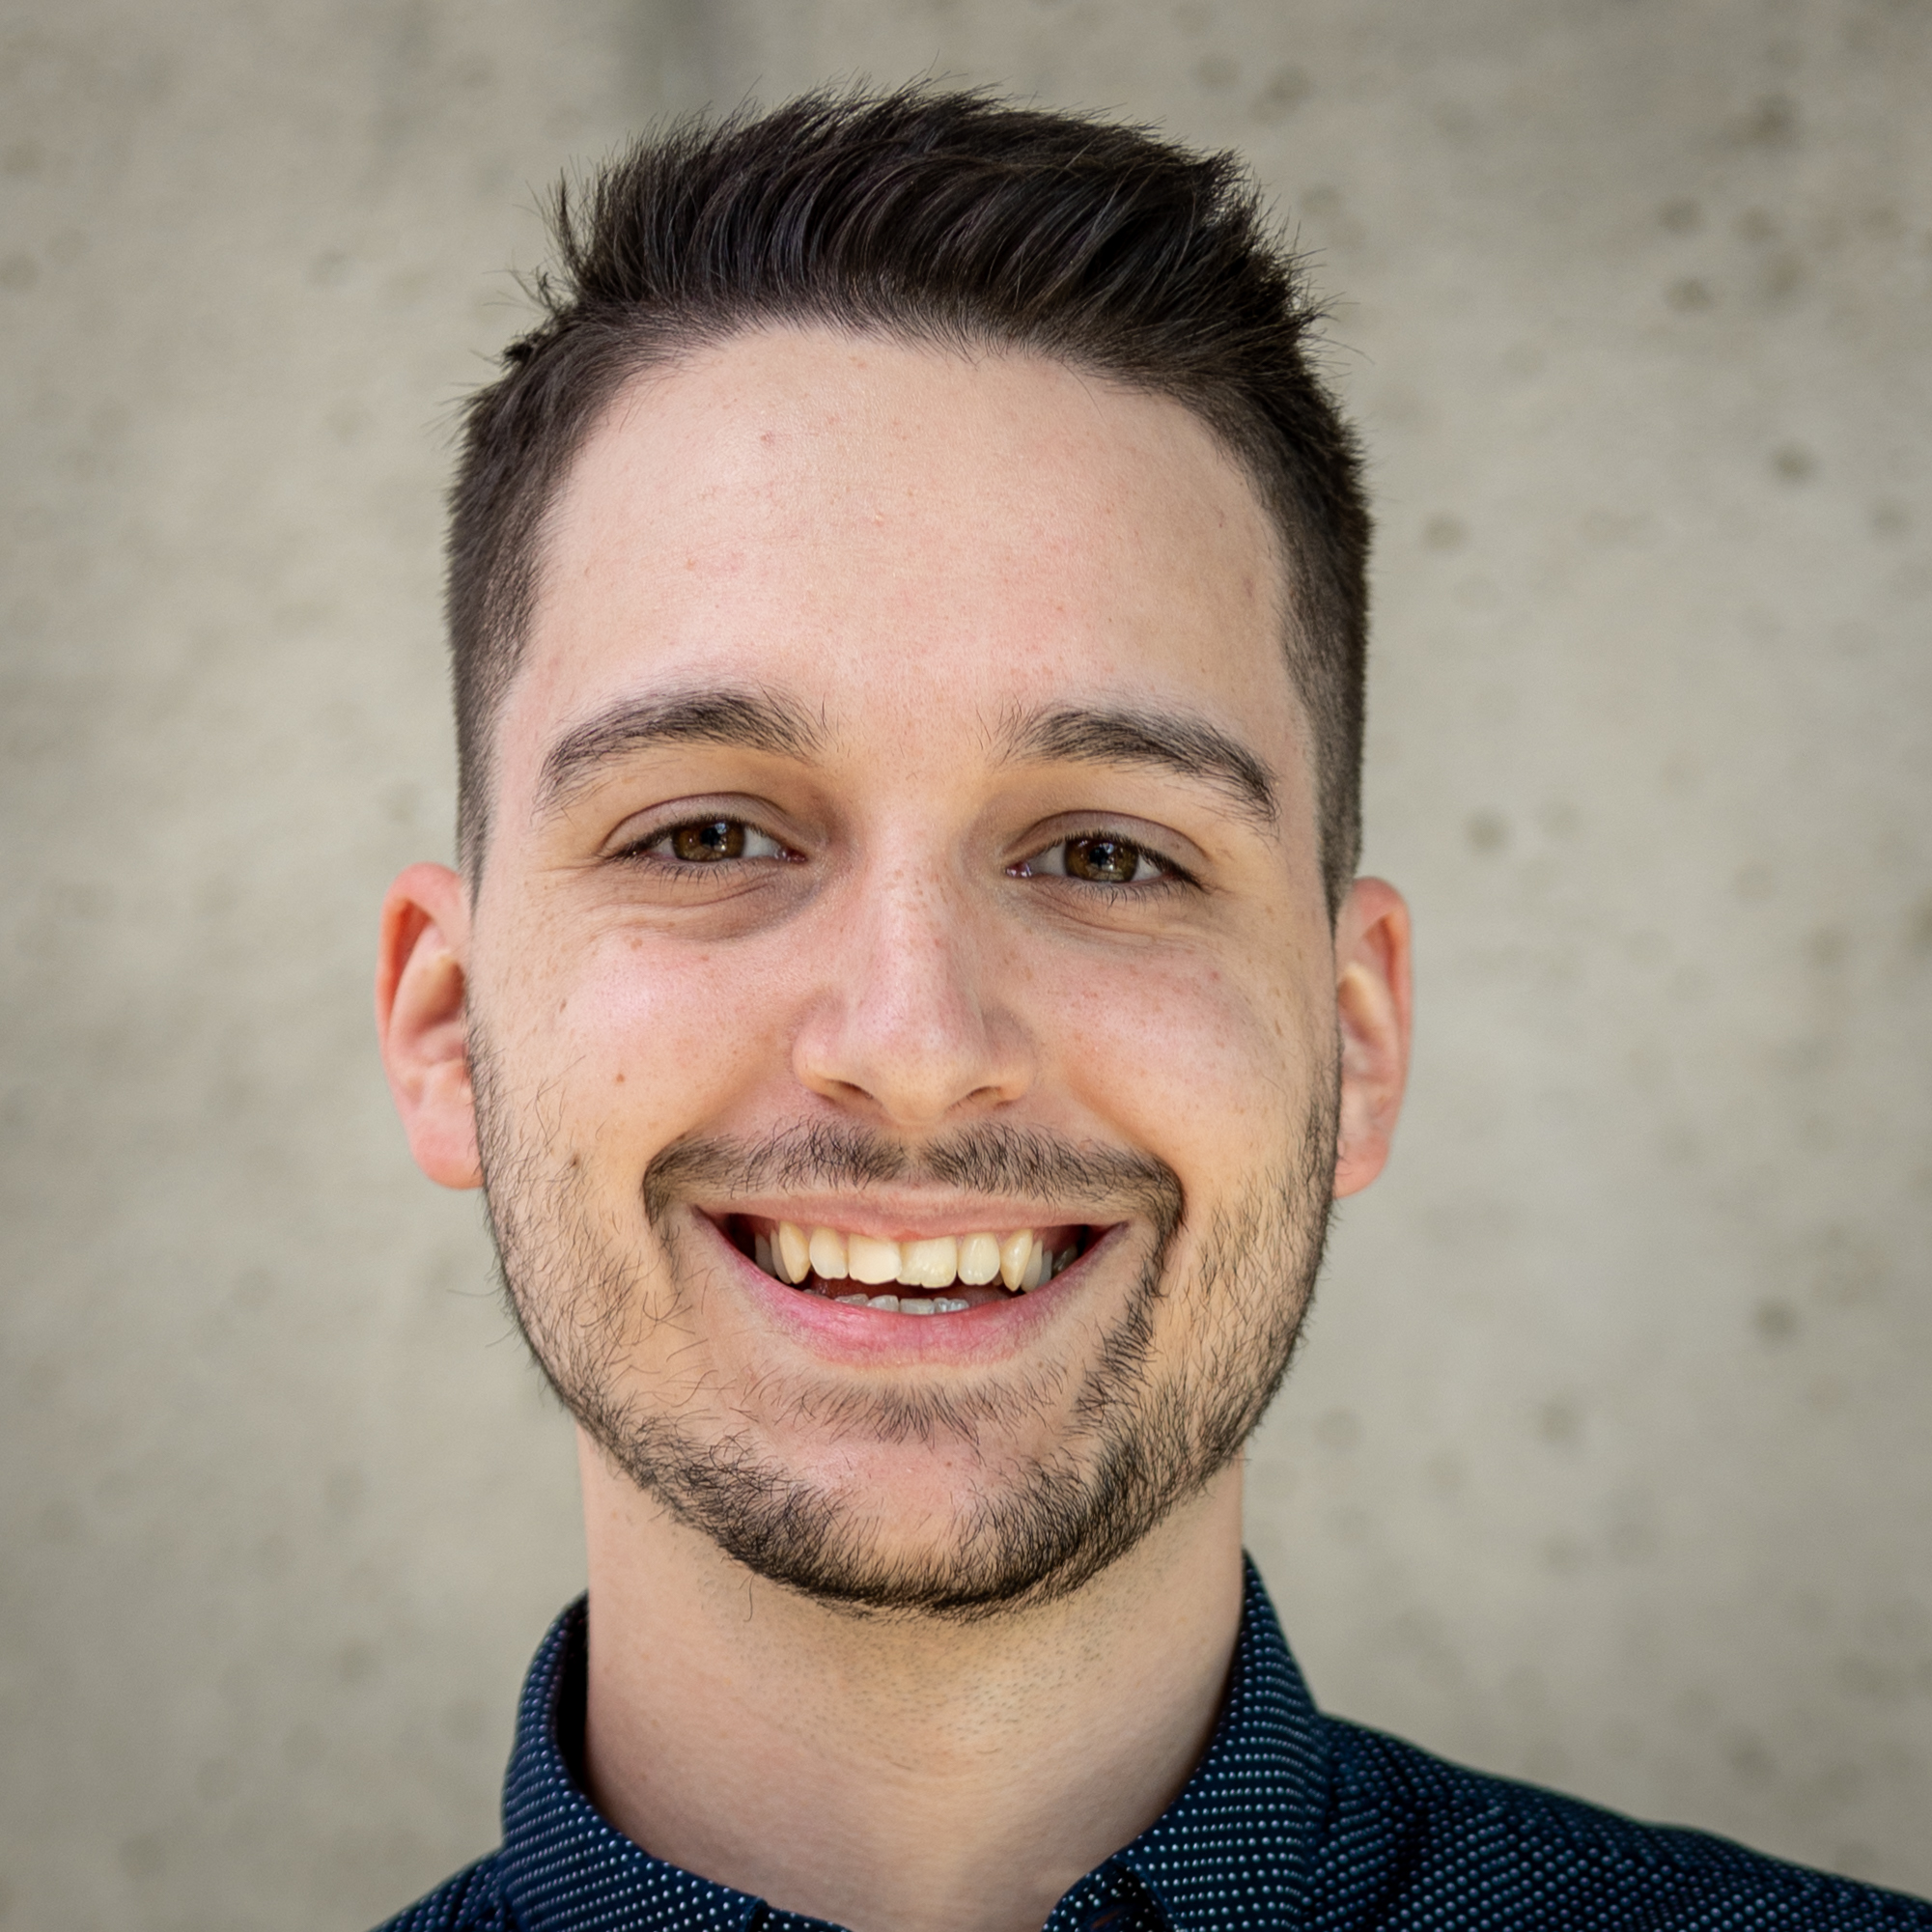
\includegraphics[width=.9\linewidth]{img/membres/Jérôme-Gelé-2.jpg} 
\end{wrapfigure}
\subsubsection*{}
% \vspace{2mm}
\textbf{Jérôme Gelé}

Onduleur

Bloc batterie

\begin{wrapfigure}[5]{r}{0.25\textwidth}
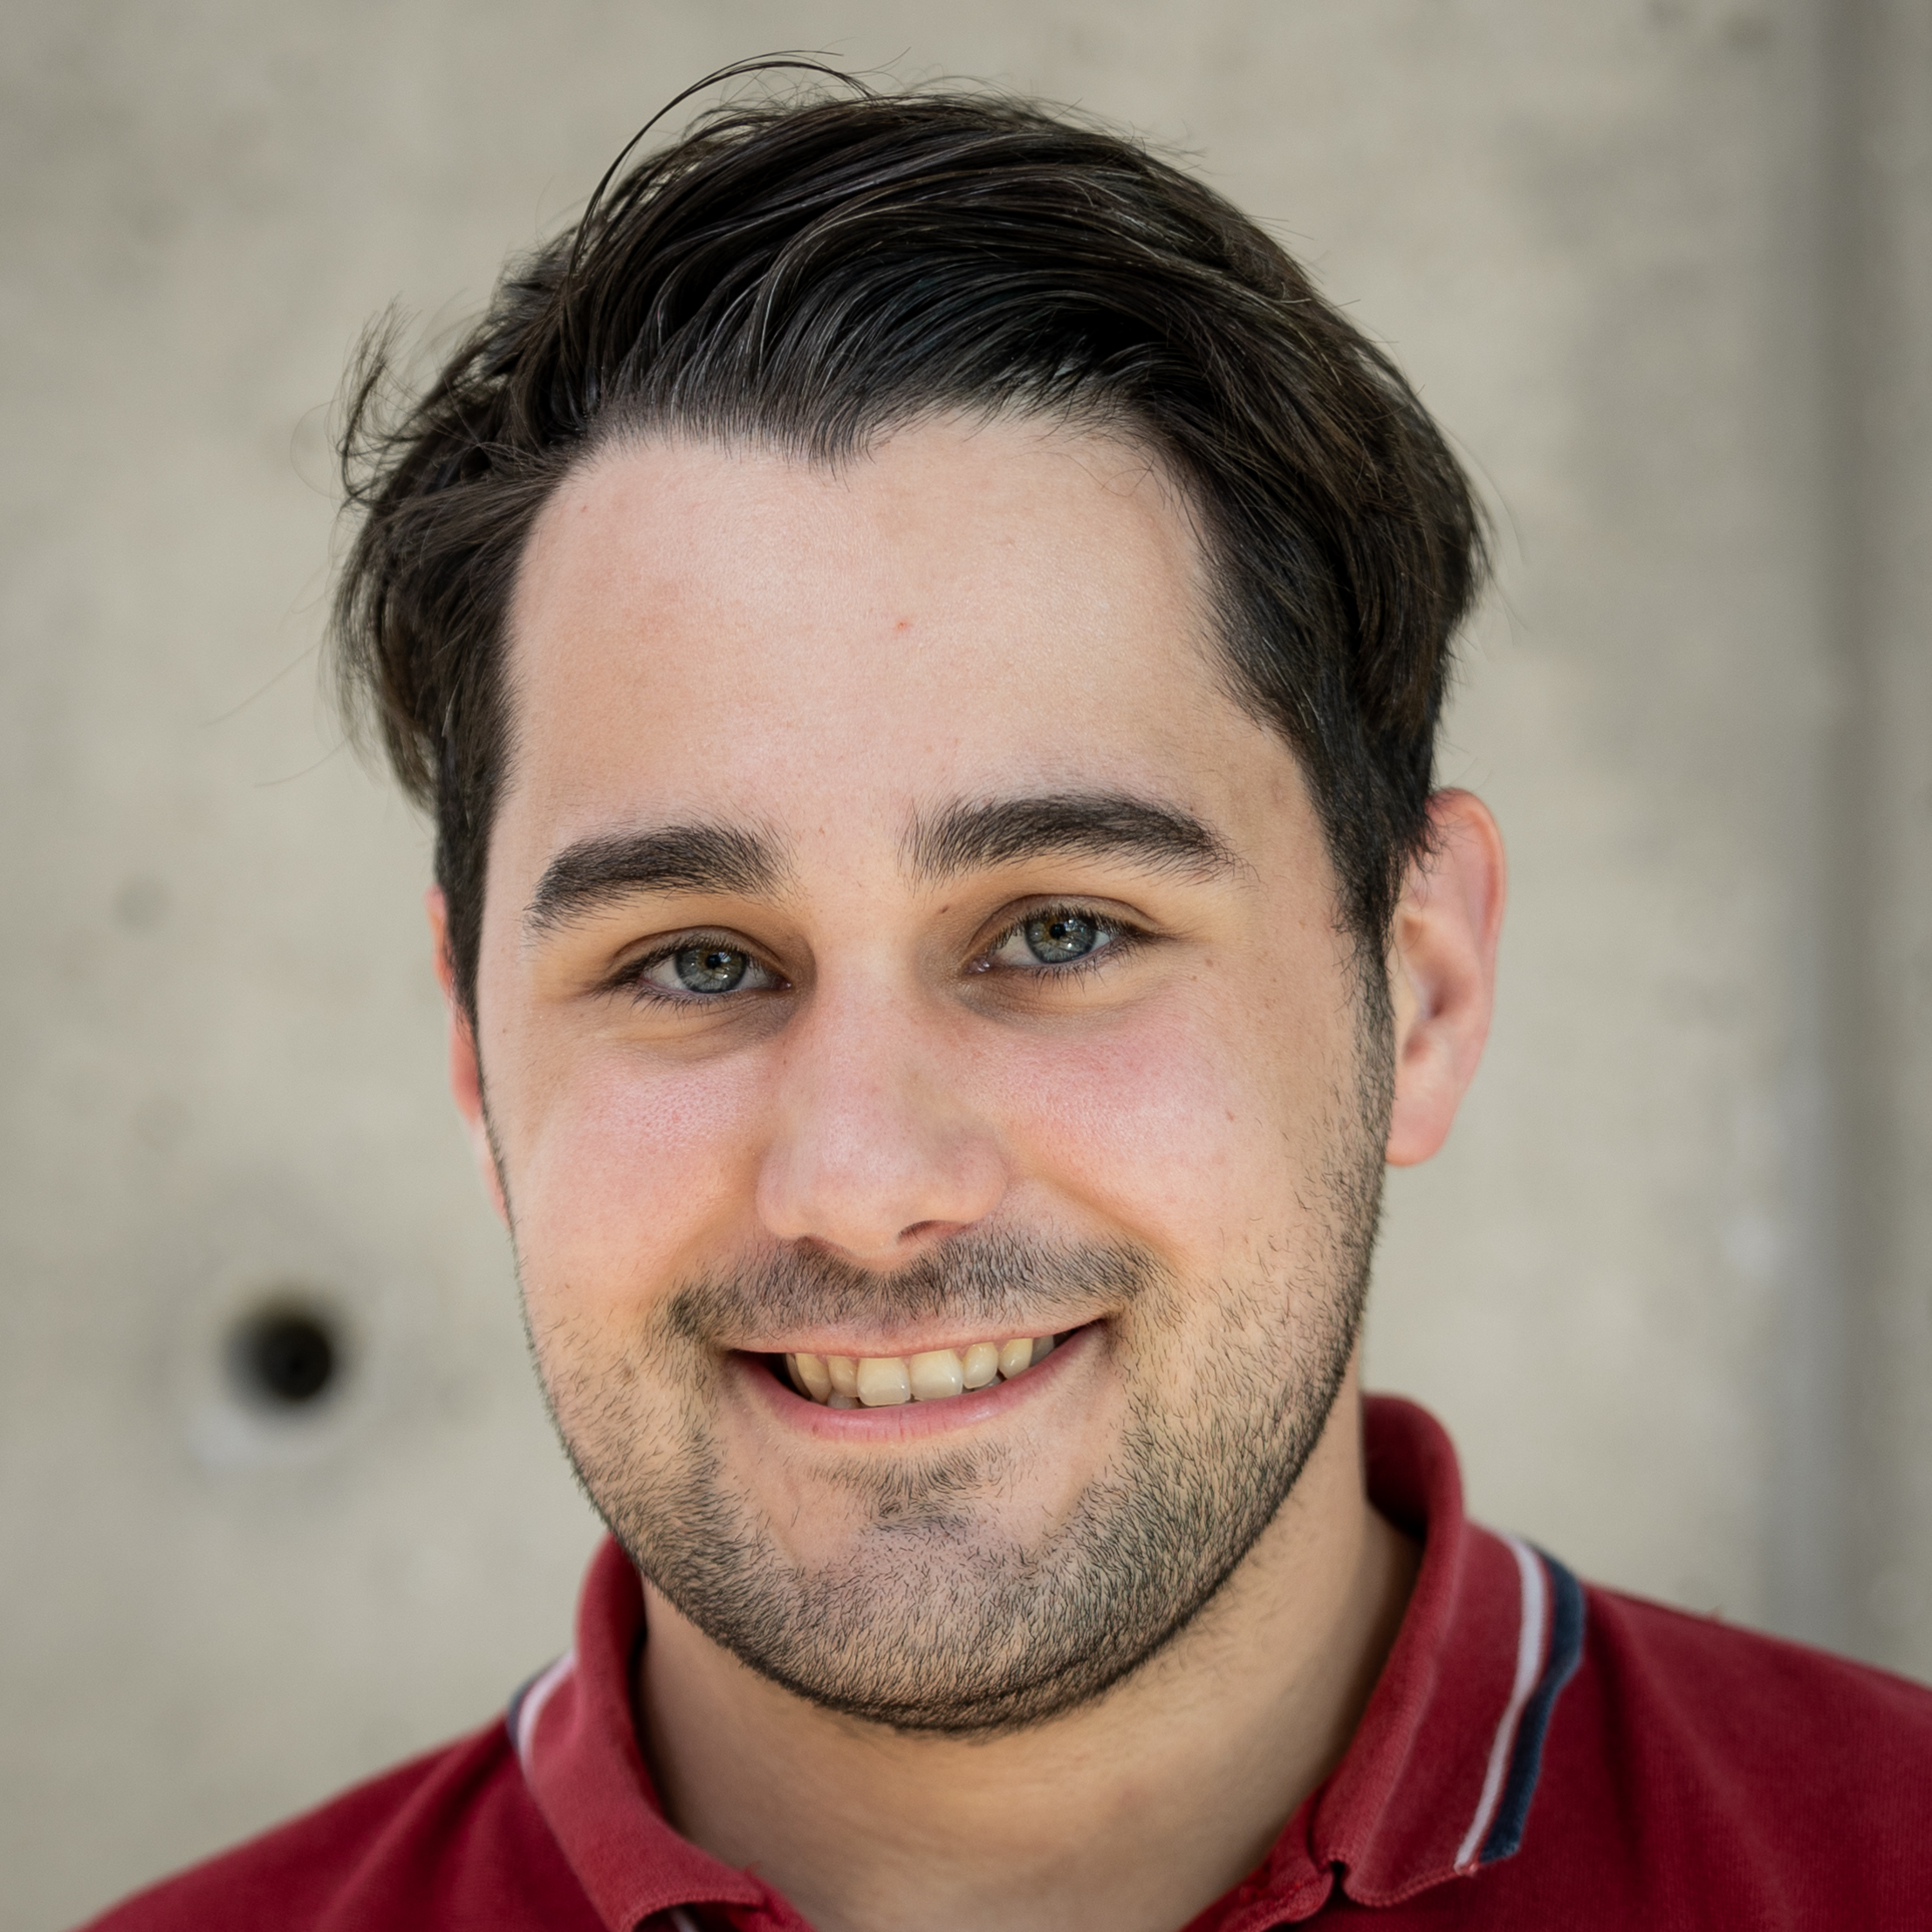
\includegraphics[width=.9\linewidth]{img/membres/Joël-Grégoire-Lagueux-1.jpg} 
\end{wrapfigure}
\subsubsection*{}
\vspace{2mm}
\textbf{Joël Grégoire-Lagueux}

Instrumentation

\begin{wrapfigure}[5]{r}{0.25\textwidth}
\includegraphics[width=.9\linewidth]{img/membres/Loïc-Poirier-2.jpg} 
\end{wrapfigure}
\subsubsection*{}
% \vspace{-2mm}
\textbf{Loïc Poirier}

Connectique
Bloc batterie


\begin{wrapfigure}[5]{r}{0.25\textwidth}
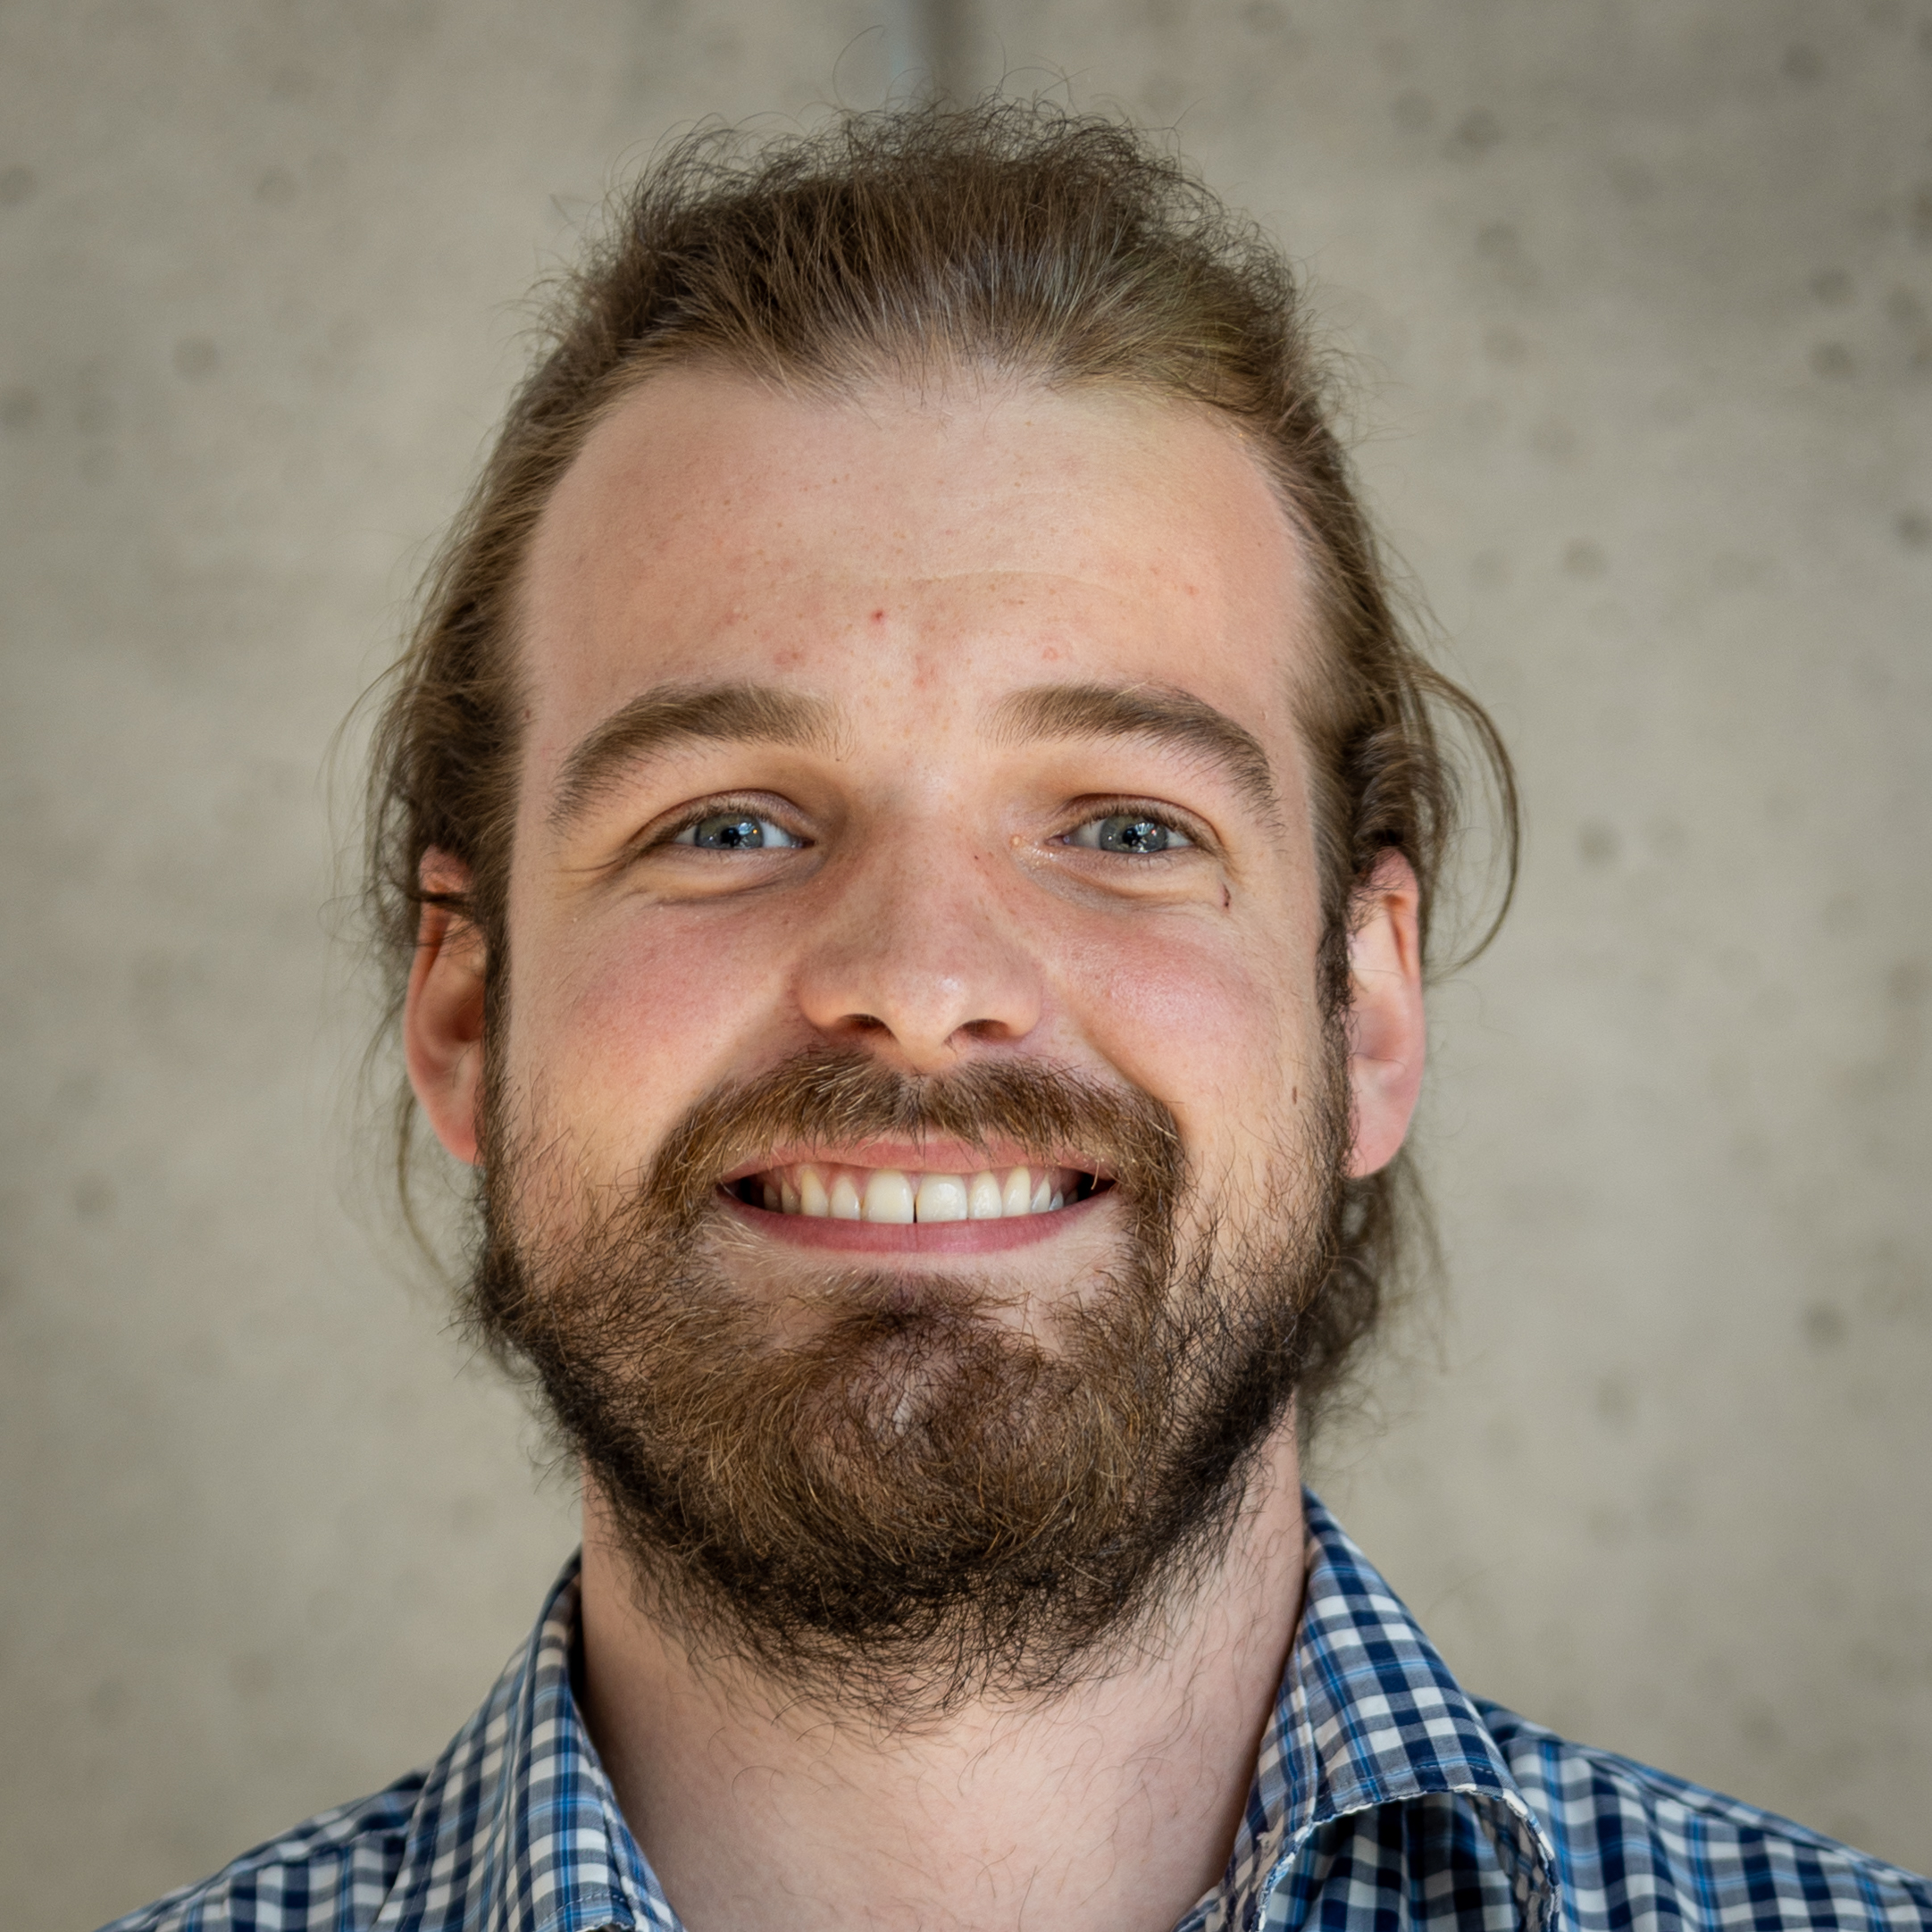
\includegraphics[width=.9\linewidth]{img/membres/Marc-Antoine-Dubreuil-2.jpg} 
\end{wrapfigure}
\subsubsection*{}
% \vspace{-2mm}
\textbf{Marc-Antoine Dubreuil}

Onduleur

Simulateur

\begin{wrapfigure}[5]{r}{0.25\textwidth}
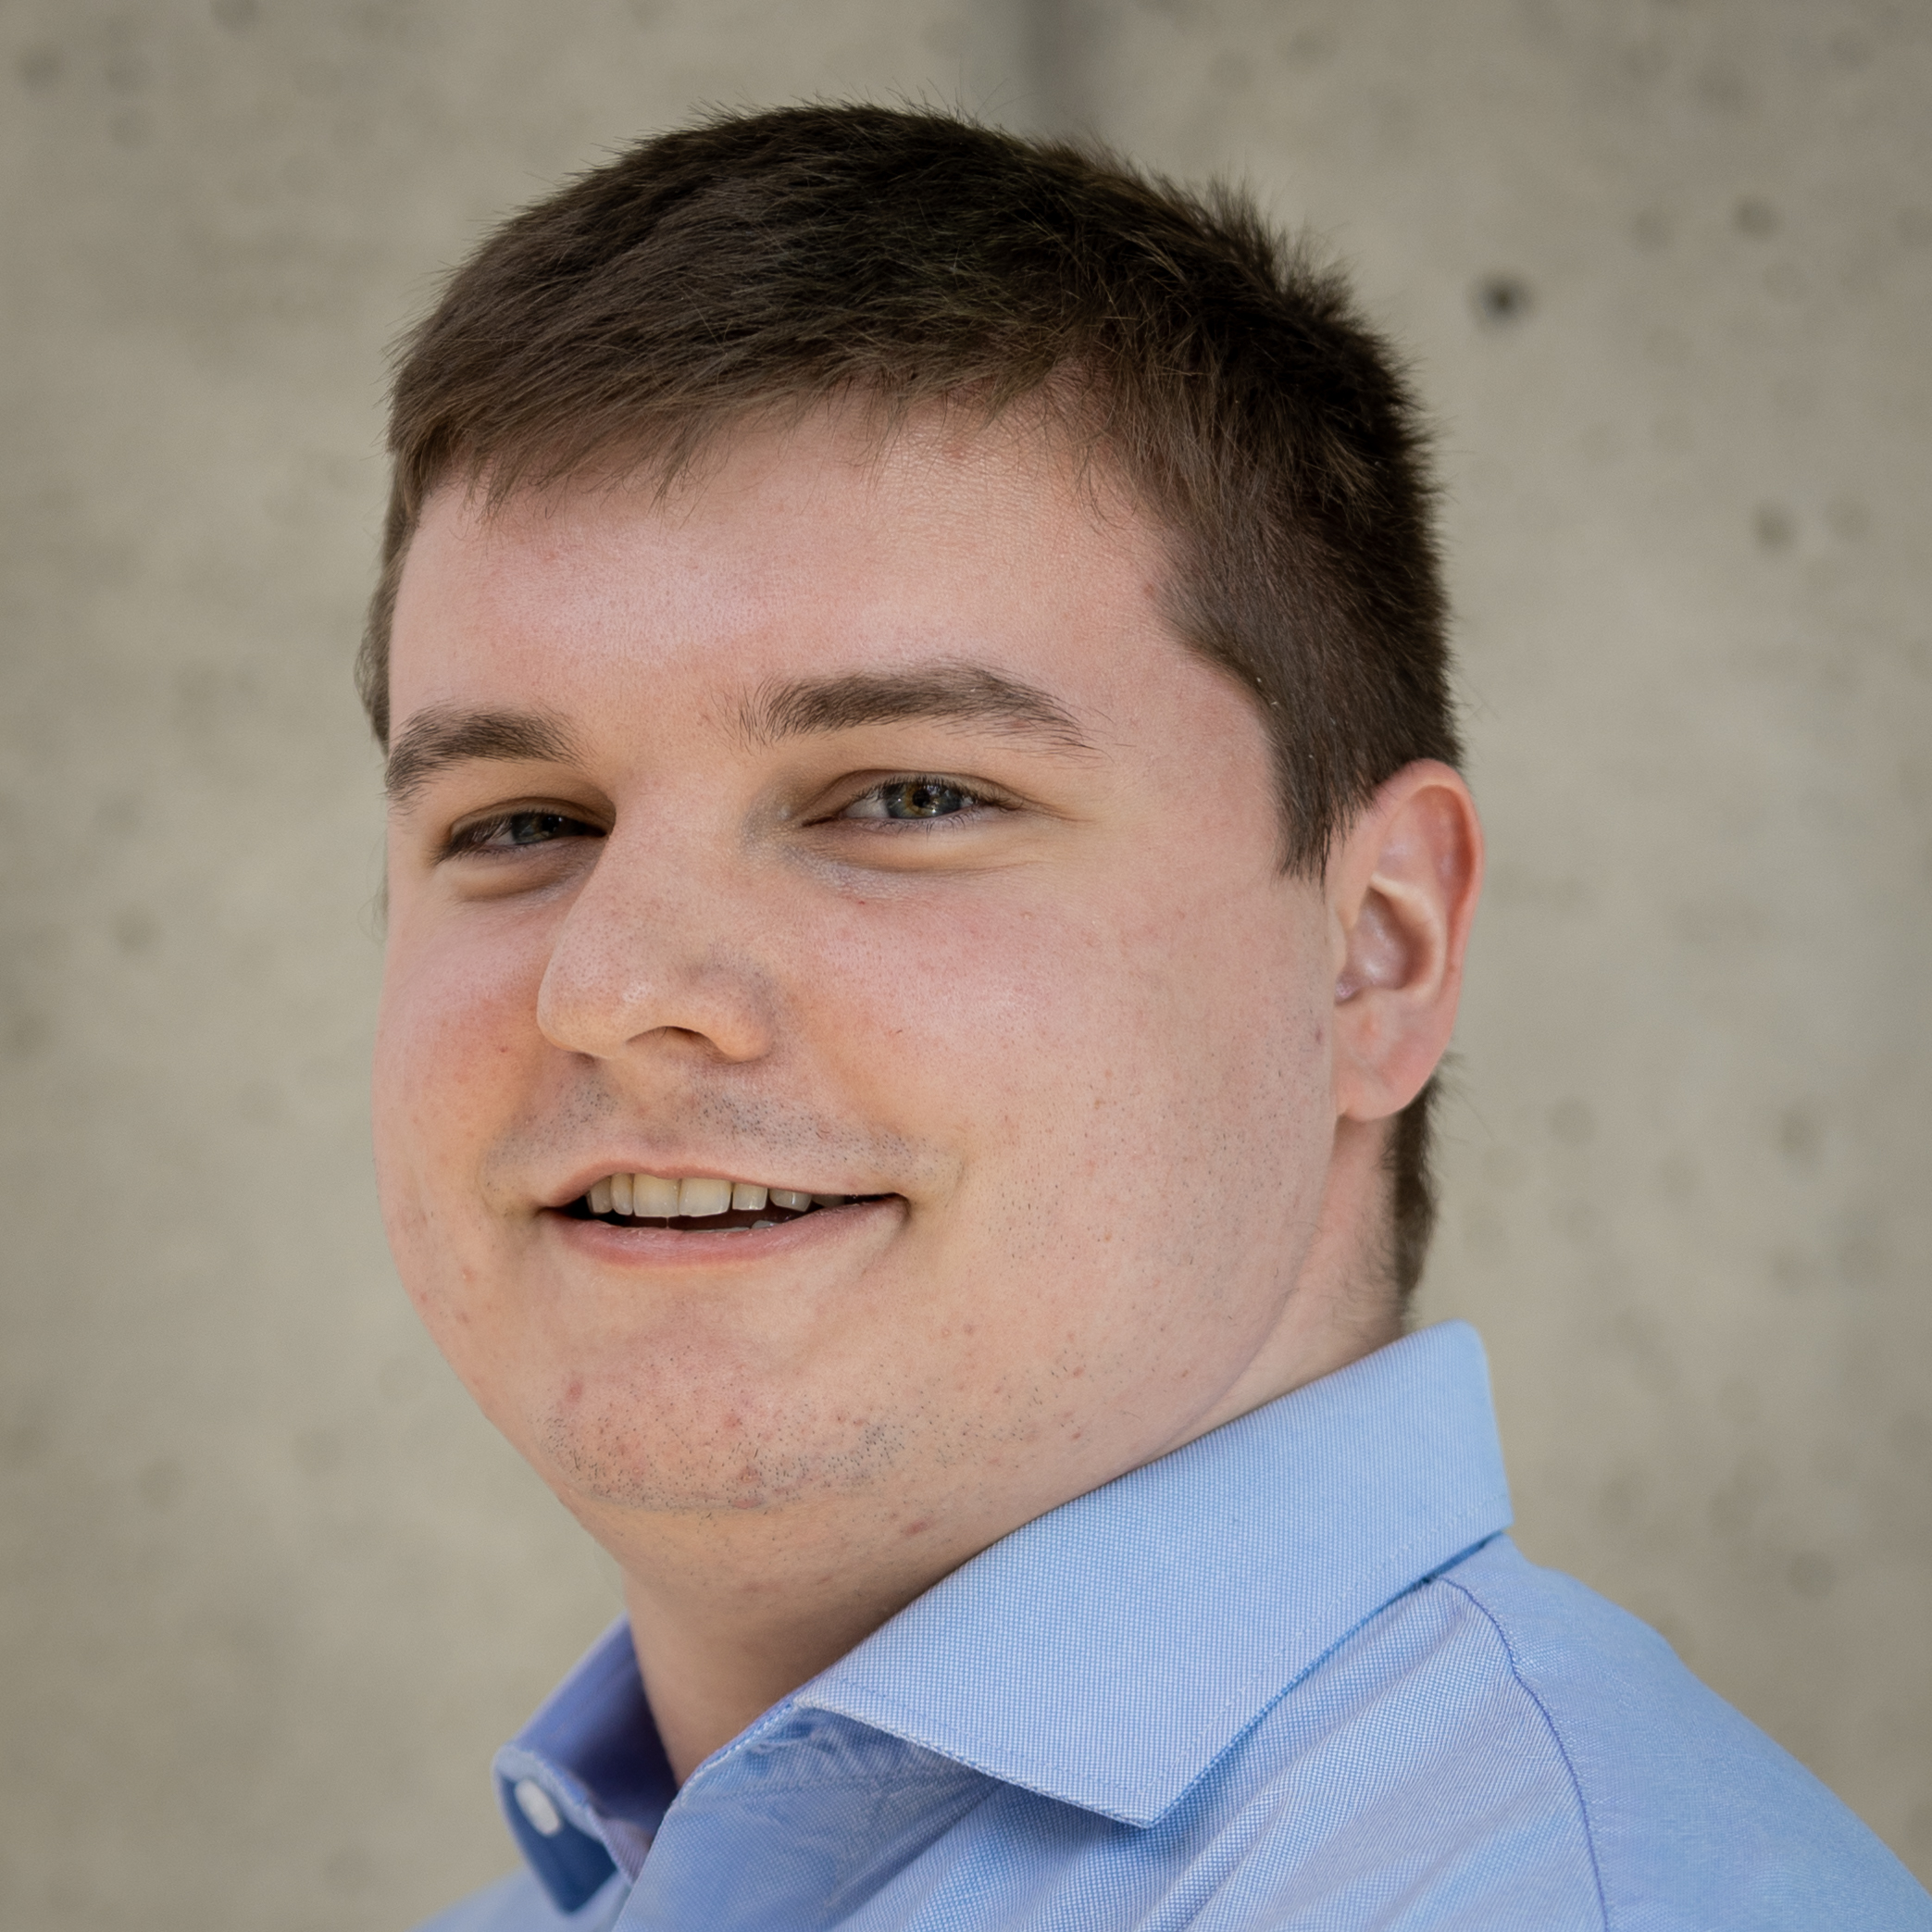
\includegraphics[width=.9\linewidth]{img/membres/Thomas-Chagnon-3.jpg} 
\end{wrapfigure}
\subsubsection*{}
\vspace{2mm}
\textbf{Thomas Chagnon}

Moteur / Transmission

\begin{wrapfigure}[5]{r}{0.25\textwidth}
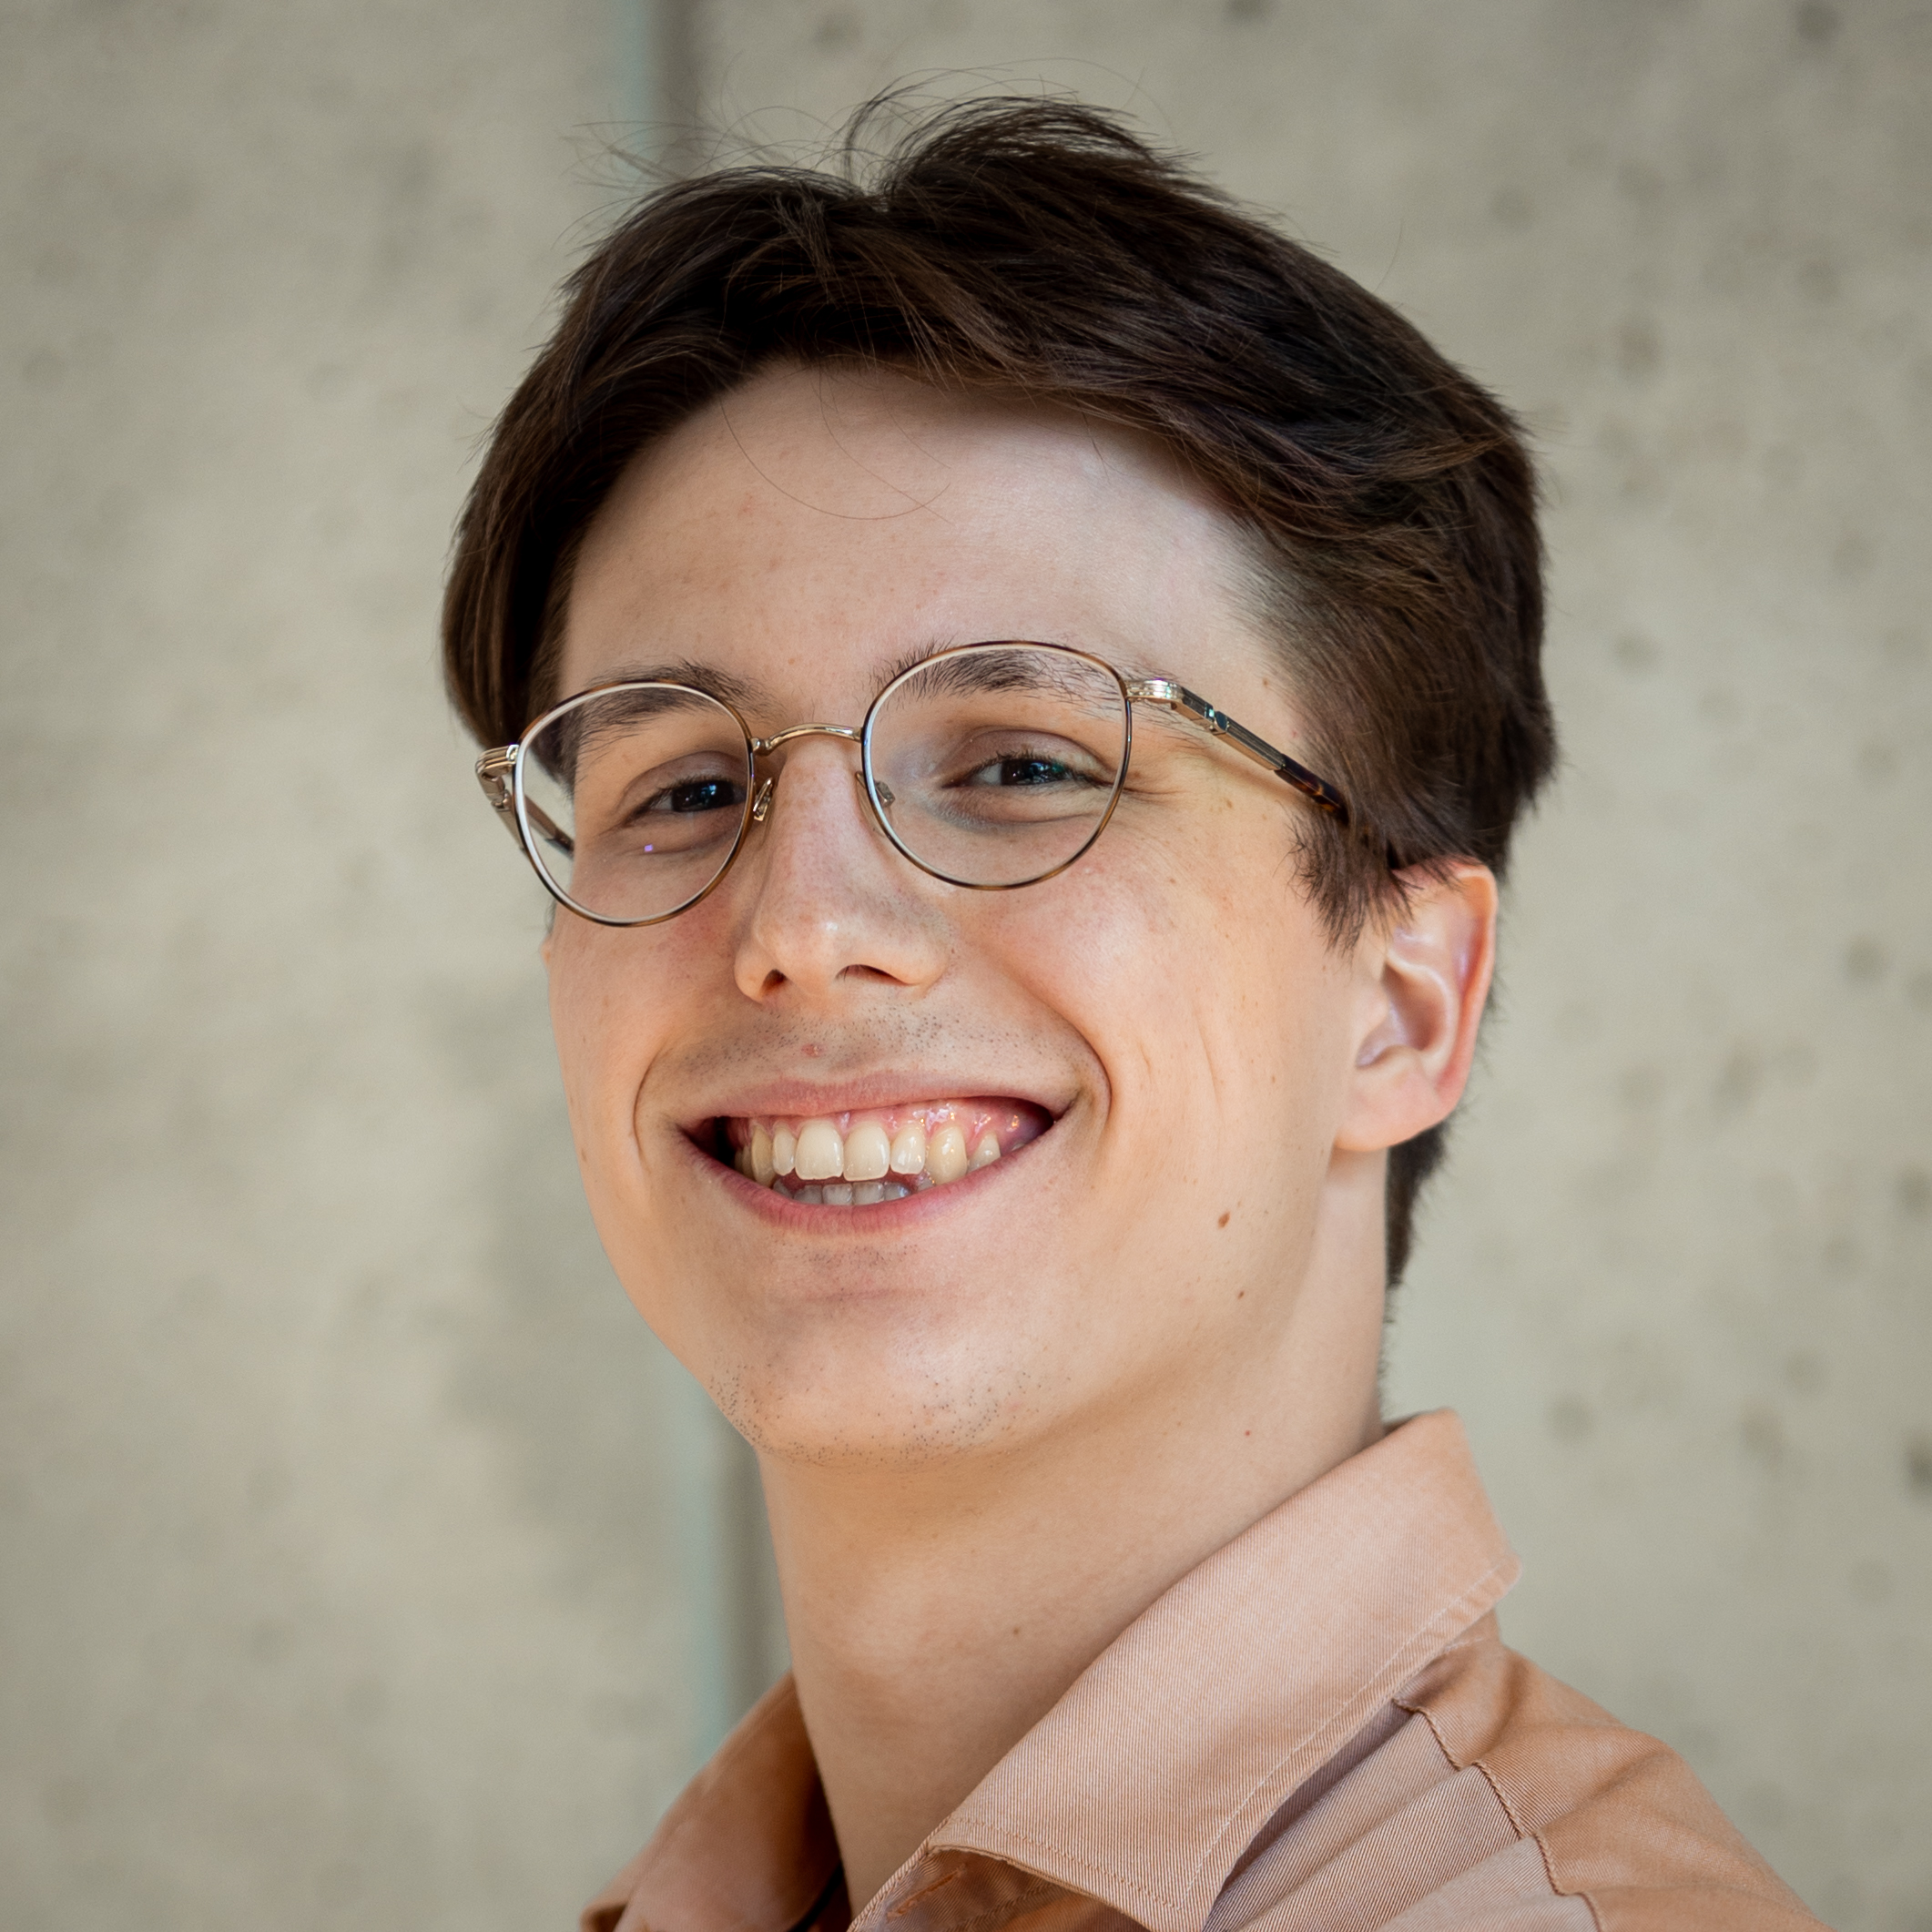
\includegraphics[width=.9\linewidth]{img/membres/Vincent-Bonneau-3.jpg} 
\end{wrapfigure}
\subsubsection*{}
\vspace{2mm}
\textbf{Vincent Bonneau}

Onduleur

Arbre d'alimentation

\begin{wrapfigure}[5]{r}{0.25\textwidth}
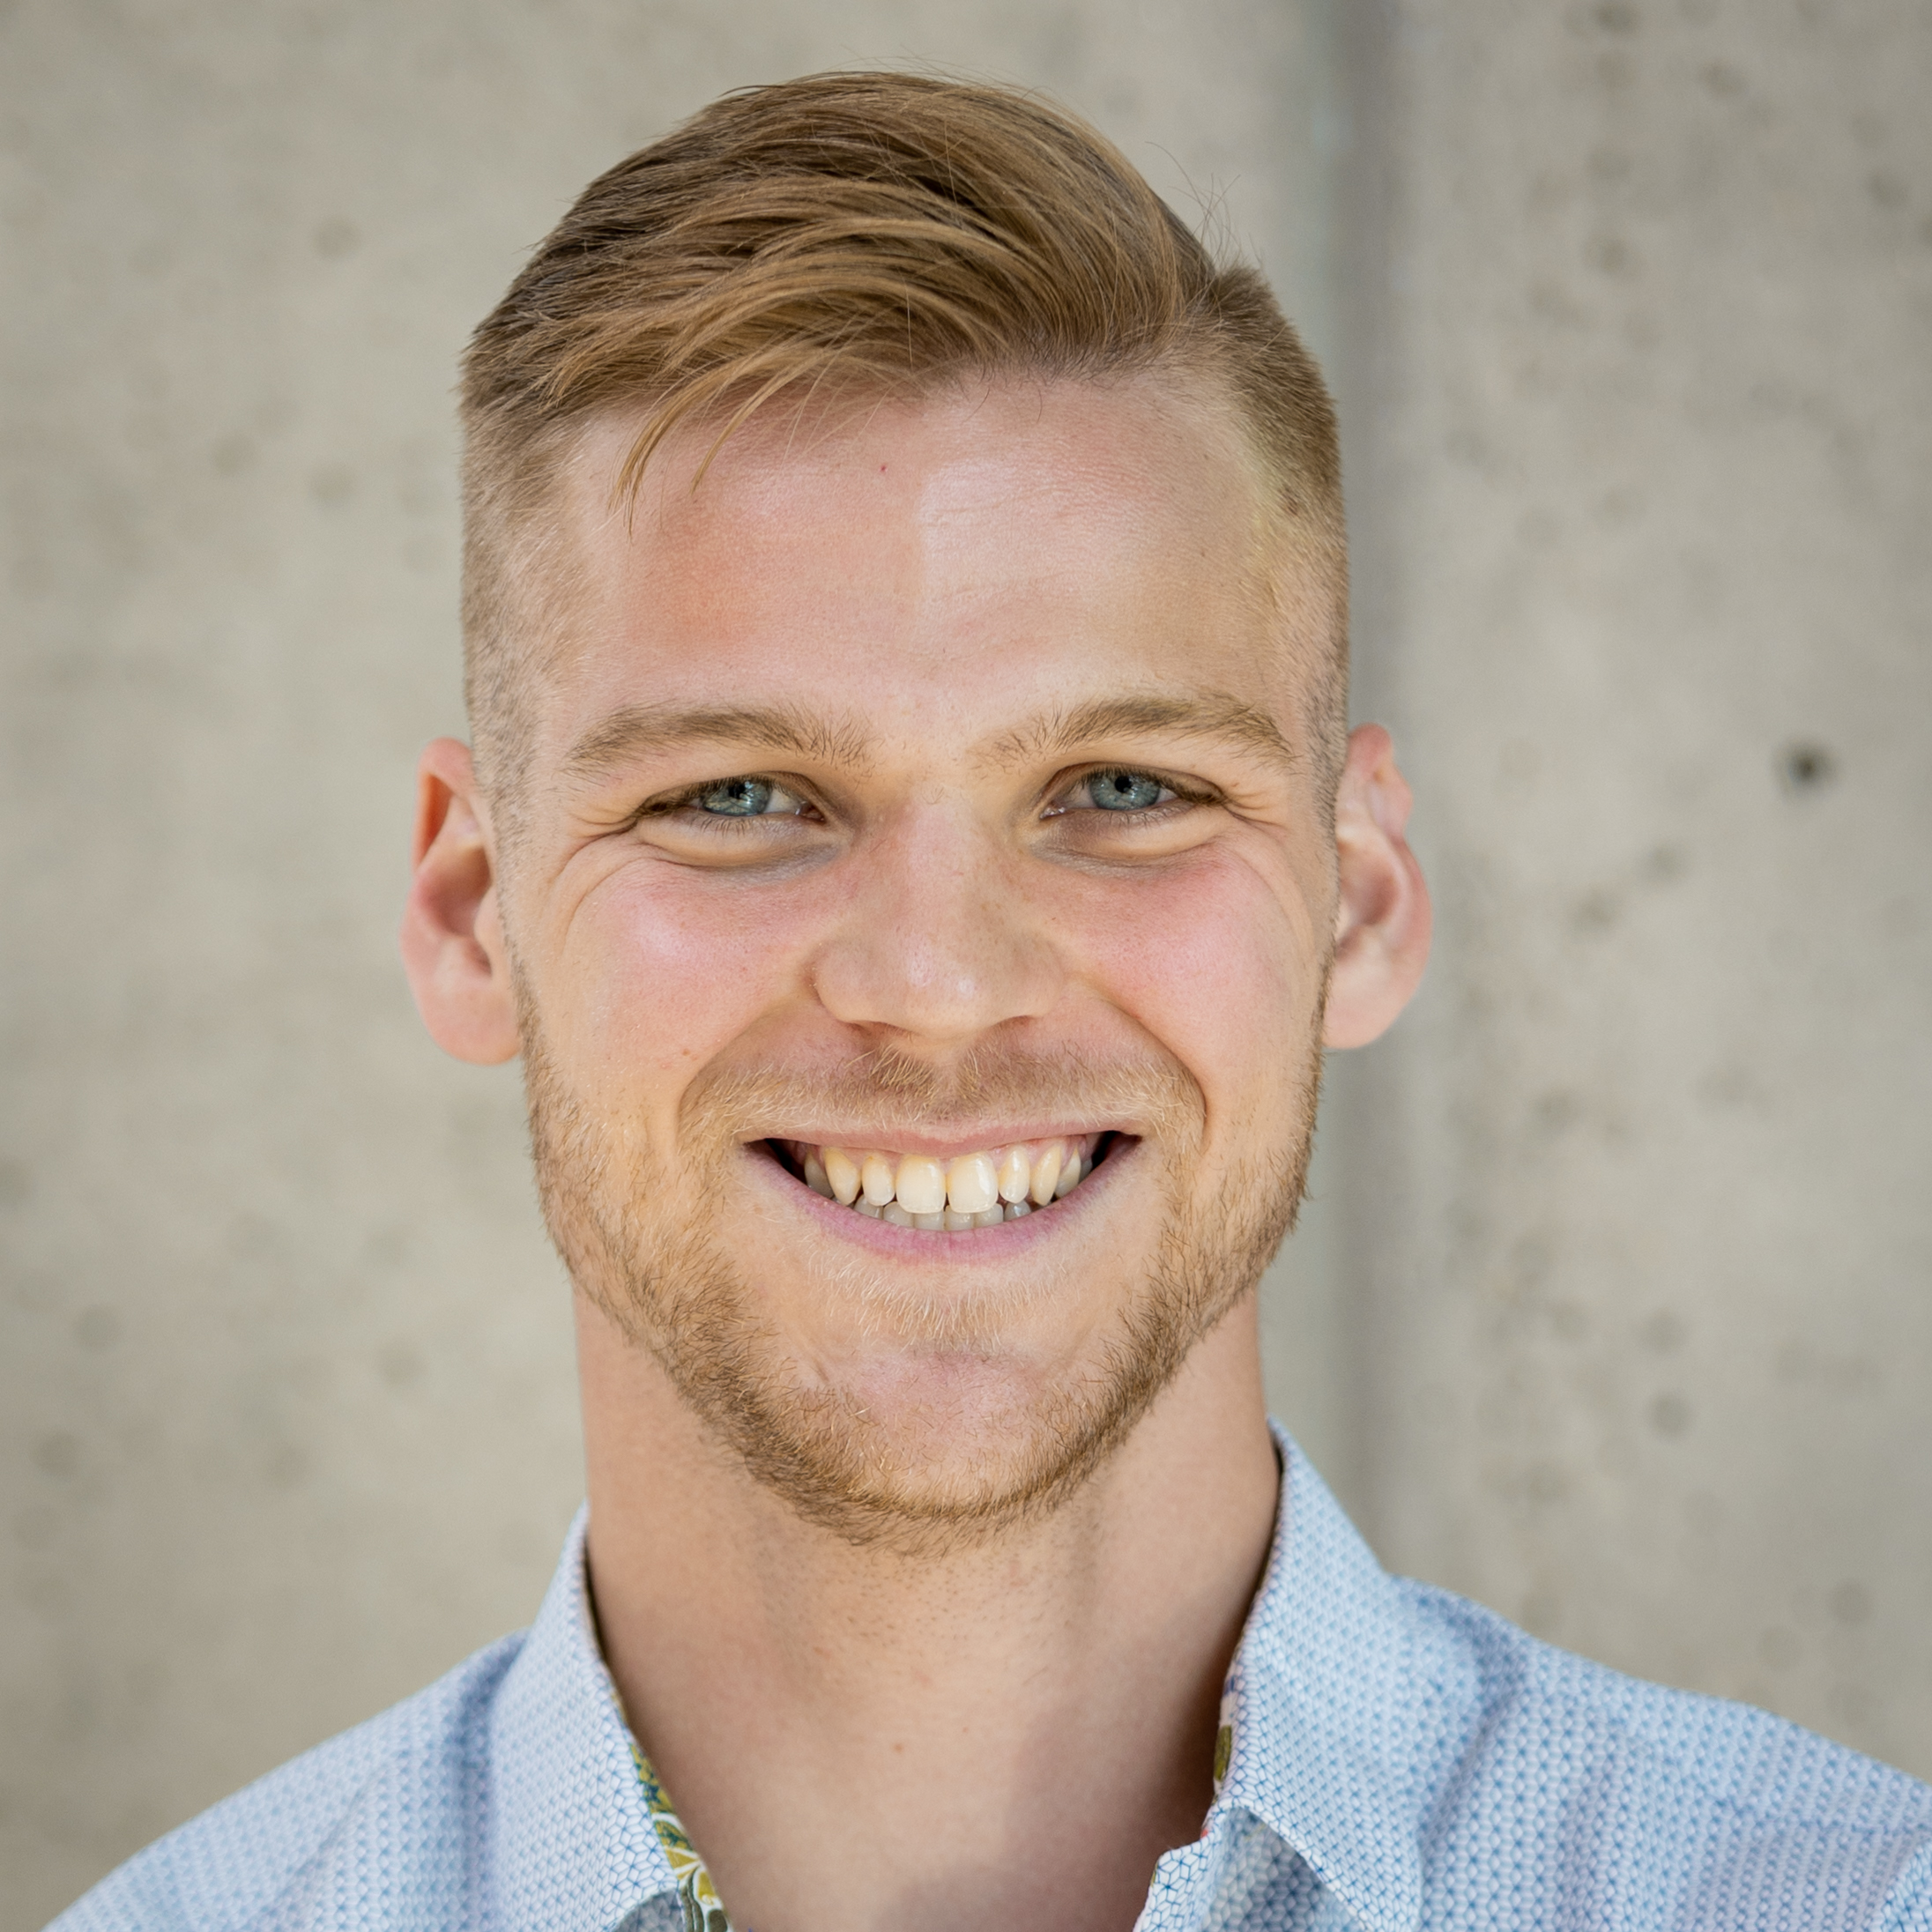
\includegraphics[width=.9\linewidth]{img/membres/Xavier-Morin-2.jpg} 
\end{wrapfigure}
\subsubsection*{}
\vspace{2mm}
\textbf{Xavier Morin}

Moteur / Transmission

Transferts thermiques

\vspace{2mm}
}


% \headerbox{Courbe en S}{name=courbe_s,column=0,span=2,below=objectif_session}{
% {
%     {
%         \hspace{0.75cm}
%         \centering
%     	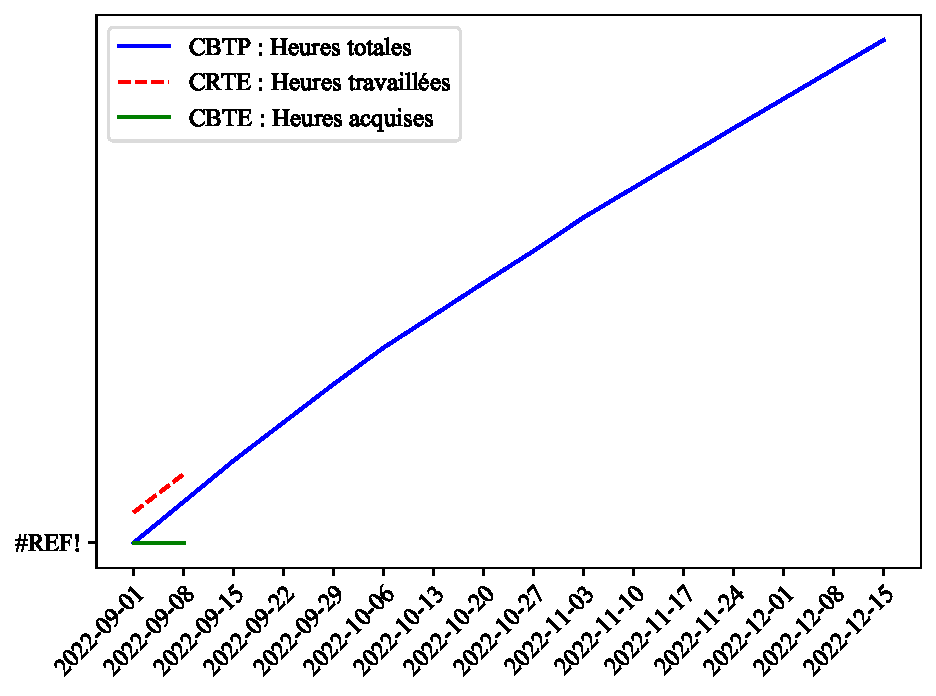
\includegraphics[width=0.9\linewidth]{img/Courbe_S.pdf}
%     }
% }

% }

\headerbox{Heures travaillées}{name=heures,column=0,span=2,below=ordre_jour}{
{
    
    {
        \hspace{0.75cm}
        \centering
    	\includegraphics[width=0.9\linewidth]{img/Heures_travaillees.pdf}
    }
    % \vspace{1.3cm}
}
}

\headerbox{Cashflow}{name=cashflow,column=0,span=2,below=heures}{
% \vspace{.6cm} % spacing vertical
\hspace{1cm}
\vspace{-4\baselineskip}
\begin{center}
    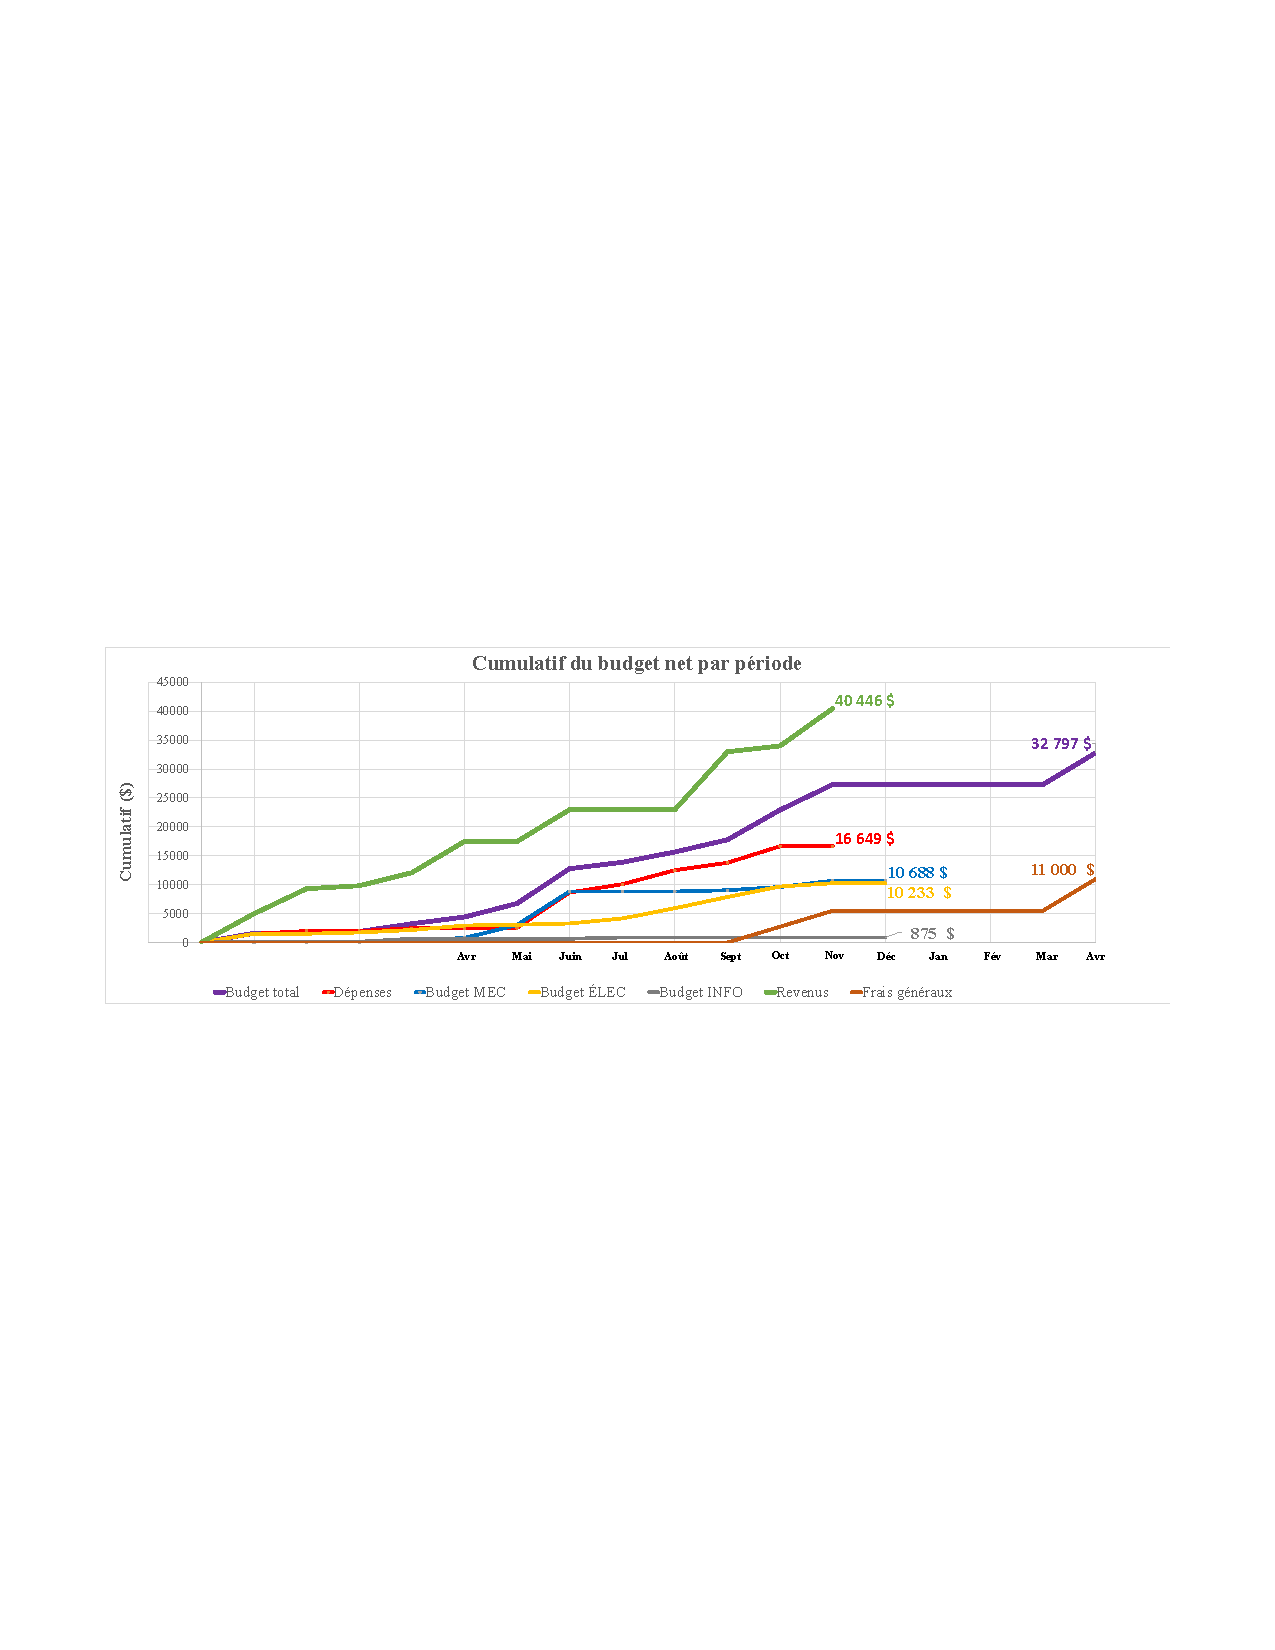
\includegraphics[width=\linewidth]{img/cashflow.pdf}
\end{center}
\vspace{-21\baselineskip}
}

\end{poster}

\begin{poster}
{
grid=false,
headerborder=open, % Adds a border around the header of content boxes
colspacing=1em, % Column spacing
bgColorOne=white, % Background color for the gradient on the left side of the poster
bgColorTwo=white, % Background color for the gradient on the right side of the poster
borderColor=Mycolor1, % Border color
headerColorOne=Mycolor2, % Background color for the header in the content boxes (left side)
headerColorTwo=Mycolor2, % Background color for the header in the content boxes (right side)
headerFontColor=white, % Text color for the header text in the content boxes
boxColorOne=white, % Background color of the content boxes
textborder=rounded, %rectangle, % Format of the border around content boxes, can be: none, bars, coils, triangles, rectangle, rounded, roundedsmall, roundedright or faded
eyecatcher=false, % Set to false for ignoring the left logo in the title and move the title left
headerheight=0\textheight, % Height of the header
headershape=rounded, % Specify the rounded corner in the content box headers, can be: rectangle, small-rounded, roundedright, roundedleft or rounded
headershade=plain,
headerfont=\Large\textsf, % Large, bold and sans serif font in the headers of content boxes
%textfont={\setlength{\parindent}{1.5em}}, % Uncomment for paragraph indentation
linewidth=1pt % Width of the border lines around content boxes
}
{}
{\textsf{{}}} % Titre vide pcq sinon ça plante
\hfill \break % Ligne vide pcq sinon ça plante

\headerbox{Objectifs bimensuels}{name=objectifs,column=0, row=0, span=3}{{{\large \textbf{Moteur / Transmission}}
\smallskip

\begin{tabularx}{\linewidth}{
    |>{\centering\hsize=0.25\hsize}X|%
    >{\centering\hsize=0.25\hsize}X|%
    >{\hsize=2.75\hsize}X|%
    >{\hsize=0.75\hsize}X|%
  }
    \hline
    \textbf{Planifié}
        &\textbf{Progrès}
        &\multicolumn{1}{>{\centering\hsize=2.5\hsize}X|}{\textbf{Objectif}}
        &\multicolumn{1}{>{\centering\hsize=0.75\hsize}X|}{\textbf{Responsable}}
    \\\hline
    100\% & 100\% & CAO moteur & Gabriel Cabana\\\hline
    100\% & 50\% & Fabriquer le gabarit de montage & Francois Paquette\\\hline
    100\% & 0\% & Decoupe lamination & Francois Paquette \\\hline
    100\% & 0\% & Machinage rotor & Francois Paquette \\\hline
    33\% & 33\% & Assemblage numérique de la transmission (SolidWorks) & Thomas Chagnon\\\hline
    75\% & 75\% & Choix des roulements à billes & Xavier Morin\\\hline
    50\% & 50\% & Calcul analytique: dimensionnement arbre, liaison entre engrenage et arbre & Xavier Morin\\\hline
\end{tabularx}
\medskip

{\large \textbf{Batterie / BMS}}
\smallskip

\begin{tabularx}{\linewidth}{
    |>{\centering\hsize=0.25\hsize}X|%
    >{\centering\hsize=0.25\hsize}X|%
    >{\hsize=2.75\hsize}X|%
    >{\hsize=0.75\hsize}X|%
  }
    \hline
    \textbf{Planifié}
        &\textbf{Progrès}
        &\multicolumn{1}{>{\centering\hsize=2.5\hsize}X|}{\textbf{Objectif}}
        &\multicolumn{1}{>{\centering\hsize=0.75\hsize}X|}{\textbf{Responsable}}
    \\\hline
    100\% & 30\% & Assemblage et test du BMS V1 & Loïc Poirier
    \\\hline
    50\% & 10\% & Conception BMS V2 & Jérôme Gelé
    \\\hline
    100\% & 80\% & Approbation du protocole d'assemblage et assemblage bloc batterie V0 & François Paquette
    \\\hline
\end{tabularx}
\medskip

{\large \textbf{Onduleur}}
\smallskip

\begin{tabularx}{\linewidth}{
    |>{\centering\hsize=0.25\hsize}X|%
    >{\centering\hsize=0.25\hsize}X|%
    >{\hsize=2.75\hsize}X|% 
    >{\hsize=0.75\hsize}X|%
  }
    \hline
    \textbf{Planifié}
        &\textbf{Progrès}
        &\multicolumn{1}{>{\centering\hsize=2.5\hsize}X|}{\textbf{Objectif}}
        &\multicolumn{1}{>{\centering\hsize=0.75\hsize}X|}{\textbf{Responsable}}
    \\\hline
    100\% & 90\% & PCB V1 DC/DC & Vincent Bonneau
    \\\hline
    100\% & 0\% & Topologie pour les autres convertisseurs & Vincent Bonneau
    \\\hline
    55\% & 25\% & Assemblage et tests PCB onduleur V1 & Marc-Antoine Dubreuil
    \\\hline
    25\% & 5\% & Conception PCB onduleur V2 & Marc-Antoine Dubreuil
    \\\hline
\end{tabularx}
\medskip

{\large \textbf{Instrumentation}}
\smallskip

\begin{tabularx}{\linewidth}{
    |>{\centering\hsize=0.25\hsize}X|%
    >{\centering\hsize=0.25\hsize}X|%
    >{\hsize=2.75\hsize}X|%
    >{\hsize=0.75\hsize}X|%
  }
    \hline
    \textbf{Planifié}
        &\textbf{Progrès}
        &\multicolumn{1}{>{\centering\hsize=2.5\hsize}X|}{\textbf{Objectif}}
        &\multicolumn{1}{>{\centering\hsize=0.75\hsize}X|}{\textbf{Responsable}}
    \\\hline
    100\% & 5\% & Commande des pièces & Joël Grégoire-Lagueux \\\hline
    100\% & 90\% & Réalisation d'un plan de tests & Joël Grégoire-Lagueux \\\hline
    % 0\% & 0\% & Assemblage,contrôle et tests & Joël Grégoire-Lagueux \\\hline
\end{tabularx}}}


\headerbox{Problèmes}{name=problemes,column=0,span=3,below=objectifs}{
\begin{tabularx}{\linewidth}{
    |>{\hsize=1.7\hsize}X|% 10% of 3\hsize 
    >{\hsize=0.5\hsize}X|% 30% of 3\hsize
    >{\hsize=0.8\hsize}X|% 30% of 3\hsize 
       % sum=0.2\hsize for 4 columns
  }
    \hline
    \textbf{Problème} & \textbf{Système} & \textbf{Responsable} \\\hline
     Redesign arbre alim & Onduleur & Vincent Bonneau \\\hline
%     Isolation du système 12V de la batterie & Onduleur & M-A Dubreuil \\\hline
  \end{tabularx}
    
    
 % Template des problèmes rencontés:
 %
 % Problème : le problème rencontré cette semaine
 % Système  : le nom ou numéro système que le problème touche ex: Simulateur ou SIM1
 % Responsable : Nom ou Initiales du ou des personnes touchées par ce problèmes ex: G.C. C.E.G.
 %
 %  \hline
 %  \textbf{Problème} & \textbf{Système} & \textbf{Responsable}\\\hline
 %  Problème & Système & Responsable \\\hline
 %  Problème & Système & Responsable \\\hline
 %  Problème & Système & Responsable \\\hline
 %  Problème & Système & Responsable \\\hline
 %  Problème & Système & Responsable \\\hline
 %  Problème & Système & Responsable \\\hline
 %  Problème & Système & Responsable \\\hline
 %
}

\headerbox{Risques}{name=risques,column=0,span=3,below=problemes}{
\begin{tabularx}{\linewidth}{
    |>{\let\newline\\\hsize=0.40\hsize}X|% 10% of 4\hsize 
    >{\hsize=0.25\hsize}X|% 30% of 4\hsize
    >{\hsize=0.25\hsize}X|% 30% of 4\hsize 
    >{\centering\arraybackslash\hsize=0.1\hsize}X|% 30% of 4\hsize 
       % sum=0.2\hsize for 4 columns
  }
    \hline
    \textbf{Risque} & \textbf{Mitigation} & \textbf{Conséquence} & \textbf{Priorité}\\\hline
    Pénurie de composantes électroniques & Commander rapidement les pièces disponibles & Redesign du concept & HAUT\\\hline
    Livraison des pièces tardive & Travailler sur les autres objectifs & Retard sur les objectifs & MOYENNE\\\hline
%    Retard important design arbre alim & Rencontre supplémentaire avec notre expert & Moins de temps de déverminage & MOYENNE\\\hline
    Intégration transmission/châssis & Rencontre avec expert SKF et système châssis & Problèmes de coaxialité arbre/roue et perpendicularité longeron & HAUT\\\hline
  \end{tabularx}
  
  
% Template pour le tableau des risques de la semaine : 

% Risque : le risque de la semaine
% Mitigation: comment mitiger le risque pour réduire ses conséquences/occurances/etc.
% Conséquence : La ou les conséquences si le risque survient
% Priorité : Priorité du risque sur une échelle de 1 à 5.  5 étant + prioritaire. La priorité est basé sur les conséquences la probablité d'occurence, etc.  
  
%  \textbf{Risque} & \textbf{Mitigation} & \textbf{Conséquence} & \textbf{Priorité}\\\hline
%    Risque & Mitigation & Conséquence & Priorité\\\hline
%    Risque & Mitigation & Conséquence & Priorité\\\hline
%    Risque & Mitigation & Conséquence & Priorité\\\hline
%    Risque & Mitigation & Conséquence & Priorité\\\hline
%    Risque & Mitigation & Conséquence & Priorité\\\hline
%    Risque & Mitigation & Conséquence & Priorité\\\hline
%    Risque & Mitigation & Conséquence & Priorité\\\hline
%    Risque & Mitigation & Conséquence & Priorité\\\hline
%    Risque & Mitigation & Conséquence & Priorité\\\hline
%    Risque & Mitigation & Conséquence & Priorité\\\hline
%    Risque & Mitigation & Conséquence & Priorité\\\hline
%    Risque & Mitigation & Conséquence & Priorité\\\hline
}

\headerbox{Citation de la semaine}{name=citation,column=0,row=0, span=3,below=risques}{
    \vspace{0.1cm}
    \textit{“Si la dernière minute n'existait pas, une quantité de choses ne serait jamais faite.”} --Anonyme
    \vspace{0.1cm} % vertical spacing
}

\end{poster}

%%%%%%%%%%%%%%%%%%%%%%%%%%%%%%%%%%%%%%%%%%%%%%%%%%

% \begin{poster}
% {
% grid=false,
% headerborder=open, % Adds a border around the header of content boxes
% colspacing=1em, % Column spacing
% bgColorOne=white, % Background color for the gradient on the left side of the poster
% bgColorTwo=white, % Background color for the gradient on the right side of the poster
% borderColor=Mycolor1, % Border color
% headerColorOne=Mycolor2, % Background color for the header in the content boxes (left side)
% headerColorTwo=Mycolor2, % Background color for the header in the content boxes (right side)
% headerFontColor=white, % Text color for the header text in the content boxes
% boxColorOne=white, % Background color of the content boxes
% textborder=rounded, %rectangle, % Format of the border around content boxes, can be: none, bars, coils, triangles, rectangle, rounded, roundedsmall, roundedright or faded
% eyecatcher=false, % Set to false for ignoring the left logo in the title and move the title left
% headerheight=0\textheight, % Height of the header
% headershape=rounded, % Specify the rounded corner in the content box headers, can be: rectangle, small-rounded, roundedright, roundedleft or rounded
% headershade=plain,
% headerfont=\Large\textsf, % Large, bold and sans serif font in the headers of content boxes
% %textfont={\setlength{\parindent}{1.5em}}, % Uncomment for paragraph indentation
% linewidth=1pt % Width of the border lines around content boxes
% }
% {}
% {\textsf{{}}} % Titre vide pcq sinon ça plante
% \hfill \break % Ligne vide pcq sinon ça plante



% \end{poster}

\end{document}